\chapter{Introduccion}
\label{ch:introduccion:primera}
La virtualización es un conjunto de técnicas hardware y/o software que permiten la ejecución
concurrente de instancias aisladas de distintos sistemas operativos en una misma plataforma
electrónica. A estos sistemas operativos se los denomina guest.
Los hipervisores fueron originalmente introducidos en el mundo IT con el objetivo de solucionar los problemas de
balanceo de carga computacional y utilización de recursos en data centers. En sus inicios, los hipervisores necesitaban cambios en los sistemas operativos guest a fin de compensar la falta de soporte hardware para el aislamiento
entre sistemas. A medida que las arquitecturas de microprocesadores han ido avanzando y añadiendo
soporte hardware para la virtualización, los hipervisores se han vuelto cada vez más habituales en los
sistemas embebidos \cite{EmbeddedWorld2018}.

La inclusión de soporte hardware para la virtualización dentro de los nuevos microprocesadores ha sido
el habilitador necesario que ha hecho que la virtualización de el salto del mundo IT a los sistemas embebidos. Las
arquitecturas más importantes de microprocesadores han evolucionado hacia la inclusión de ése soporte hardware.
Como ejemplos notables están la tecnología de virtualización de Intel  (Intel VT-x), las extensiones de virtualización de la arquitectura ARM y MIPS VZ extensions.
Este soporte hardware, lo que aporta es un modo de ejecución nuevo, con mayores privilegios que el tradicional modo
supervisor, e input-output memory management units (\acrshort{IOMMU}) con el objetivo de aislar periféricos entre sistemas operativos guest. La versión de intel de \acrshort{IOMMU} recibe el
nombre de VT-d y en la mayoría de los sistemas ARM existe un ``System \acrshort{MMU}'' equivalente. En los data center, el \acrshort{IOMMU} se denomina habitualmente ``Single Root Virtualization'' o SRV.\\[1cm]
\textbf{Casos de uso}
\begin{itemize}
	\item Sistemas de criticidad mixta\\
	El caso de uso más habitual de los hipervisores es el de consolidar diferentes cargas de computación en una única
	plataforma a fin de reducir el tamaño, consumo y coste de un sistema. Los sistemas operativos guest, al estar aislados unos de otros, hace que parezca que están ejecutándose en máquinas físicamente distintas. En el mundo de la automoción por ejemplo,
	se dan casos en los que se combina el clúster de instrumentación o dashboard con el sistema de infoentretenimiento del vehículo (\acrshort{IVI}) en una sola unidad de control electrónica (ECU). El clúster de instrumentación está desarrollado normalmente sobre un sistema operativo de tiempo real (\acrshort{RTOS}), mientras que el \acrshort{IVI} habitualmente requiere de un sistema operativo Linux u otro sistema operativo de propósito general (\acrshort{GPOS}). La criticidad mixta se refiere a que los requisitos de tiempo real y seguridad del clúster de instrumentación no pueden ser cubiertos por un \acrshort{GPOS} y las librerías multimedia necesarias para el sistema de infotainment son costosas de portar a un \acrshort{RTOS}. Por lo tanto integrar estas funcionalidades a la vez en un único sistem operativo no es viable a día de hoy. Un hipervisor con características de tiempo real y seguridad es capaz de hacer que ambos sistemas se puedan ejecutar en un mismo procesador. Esto permite un ahorro de costes significativo al necesitar una única tarjeta electrónica para todo el sistema.
	\item Sistemas Legacy\\
	A medida que los sistemas evolucionan con el tiempo, a menudo es necesario moverse a nuevos entornos o sitemas operativos a fin de añadir funcionalidades. Preservar la funcionalidad ya existente y certificada del sistema requeriría portar todo el código a la nueva plataforma y probar todo de nuevo. La virtualización permite la ejecución concurrente de la funcionalidad tal cual fue certificada junto con el nuevo software que añade funcionalidades en el mismo procesador. Un ejemplo de esto es la radio definida por software. Los requisitos pueden ir cambiando con el tiempo y pasar de un simple interfaz \acrshort{LCD} a un interfaz gráfico de usuario (\acrshort{GUI}). La parte de radio puede ser muy costosa de recertificar. Utilizando virtualización, se puede mantener la parte de radio tal cual fue certificada y añadir un sistema operativo con una librería moderna de \acrshort{GUI}.
	Este caso de uso es el más comun en los sistemas muy sensibles al coste.\\[1cm]
\end{itemize}
\textbf{Capacidades de los hipervisores}\\
Todos los hipervisores proporcionan mecanismos de compartición de recursos en sistemas on chip (\acrshort{SoC}), pero difieren en la profundidad y el soporte hardware.
\begin{itemize}
	\item Compartición de memoria\\
	El hipervisor más básico en un \acrshort{SoC} solo proporciona la compartición de memoria. Cada sistema guest se le asigna una CPU. El hipervisor configura el sistema de memoria virtualizada del \acrshort{SoC}, con el objetivo de restringir cada CPU a una parte del mapa de memoria, incluyendo memoria RAM y periféricos. Esto permite a distintos sistemas operativos guest ejecutarse en un único \acrshort{SoC} con periféricos disjuntos y acceso seguro a \acrshort{RAM}.
	\item Compartición de CPU\\
	Un hipervisor más sofisticado permite la compartición de núcleos de CPU individuales utilizando multiplexado en el tiempo. Esto posibilita a las diferentes cargas computacionales disponer de todos los recursos de la CPU en situaciones de alta demanda y distribuir ese acceso en función de la prioridad. Por ejemplo, en el caso de la coexistencia de un \acrshort{RTOS} y un \acrshort{GPOS}, el \acrshort{RTOS} tiene normalmente mayor prioridad en las CPUs, mientras que al \acrshort{GPOS} se le garantiza un tiempo mínimo de ejecución. El \acrshort{GPOS} tiene acceso completo mientras que el \acrshort{RTOS} está inactivo. Hay que tener en cuenta que los hipervisores que permiten la compartición de CPU deben de ser diseñados con compartamiento en tiempo real, y normalmente están basados en algún \acrshort{RTOS}.
	\item Compartición de periféricos\\
	Otra de las características de los hipervisores es la compartición de periféricos tales como dispositivos de almacenamiento, interfaces de red o \acrshort{GPU}s. Los sistemas embebidos suelen ser sensibles al coste y por tanto el poder compartir un dispositivo \acrshort{eMMC} es casi un requisito. Hay diferentes técnicas para implementar la compartición de periféricos que se comentarán más adelante.
\end{itemize}

Los hipervisores se clasifican habitualmente en dos tipos \cite{Popek1974}\cite{hyper_review}:
\begin{itemize}
\item \textbf{Tipo 1 o baremetal}: en este grupo están los hipervisores que se ejecutan directamente sobre
la plataforma electrónica sin ningún otro software de por medio del tipo sistema operativo u
otros controladores. Tienen acceso directo al hardware y gestionan los diferentes sistemas guest. Estos hipervisores se caracterizan por ser una pequeña capa software que proporciona el entorno necesario para que los sistemas guest se puedan ejecutar. Se utilizan habitualmente en sistemas embebidos ya que son los que menos impacto tienen sobre el rendimiento del sistema. Los primeros hipervisores que desarrollo IBM en los años 60 son de este tipo \cite{hyper_review}\\
\begin{figure*}[h]
	\centering
	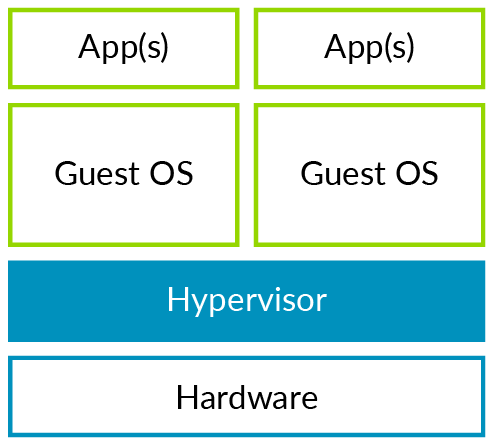
\includegraphics[width=0.55\textwidth]{recursos/type1_hyp.png}
	\caption{Hipervisor de tipo 1}
	\label{fig:hyper_type1}
\end{figure*}
\item \textbf{Tipo 2}: estos hipervisores suelen instalarse sobre un sistema operativo convencional (host) de base y
acceden a los recursos del sistema (memoria, procesadores, almacenamiento, red, etc.) a
través de él. Su funcionamiento es parecido al de cualquier otro programa que se ejecuta en el sistema host. Son responsables de abstraer al sistema guest del sistema host donde se están ejecutando. Algunos ejemplos de estos hipervisores son los populares VMWare y VirtualBox. Estos hipervisores tienen un impacto notable en el rendimiento, ya que todo el acceso a los recursos del sistema se hace a través del sistema host.
\begin{figure*}[h]
	\centering
	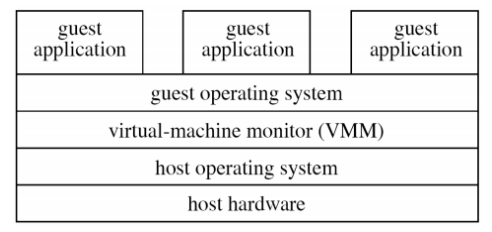
\includegraphics[width=0.55\textwidth]{recursos/type2_hyp.png}
	\caption{Hipervisor de tipo 2}
	\label{fig:hyper_type2}
\end{figure*}
\\
\end{itemize}

En los sistemas virtualizados el hipervisor es denominado también Monitor de Máquinas Virtuales o \acrshort{VMM} en sus siglas en inglés. Como se ha mencionado anteriormente, es la parte encargada de ofrecer una versión virtualizada de los recursos del sistema y gestionar las distintas máquinas virtuales en funcionamiento. Al virtualizar los recursos del sistema y las APIs, el hipervisor es capaz de ejecutar diferentes máquinas virtuales simultaneamente utilizando tecnologías de virtualización que se pueden dividir en las siguientes modalidades \cite{hyper_perf_arm}:
\begin{itemize}
	\item Virtualización completa: En este tipo de virtualización, el hypervisor simula los recursos (CPU, memoria, periféricos, ...) de tal forma que se pueden ejecutar sistemas operativos guest sin ningún tipo de modificación. El sistema operativo guest es un dominio con privilegios de ejecución limitados. La virtualización completa utiliza la conversión binaria para traducir las operaciones que requieren de privilegios en un bloque equivalente de operaciones sin privilegios que pueden ejecutarse directamente en la CPU, produciendo el mismo resultado que las operaciones originales.\\
	En este modo de virtualización ni el hardware ni el sistema operativo requieren de ningún tipo de modificación.
	\item Paravirtualización: esta técnica de virtualización resulta en un impacto menor en el rendimiento del sistema que la virtualización completa. En la paravirtualización, el sistema operativo guest ha de ser modificado con objeto de utilizar las denominadas \textit{hypercalls} en lugar de las instrucciones que requieran privilegios. Al igual que una llamada al sistema (syscall) es una software trap de la aplicación al sistema operativo, una \textit{hypercall} es una software trap de un sistema operativo guest al hipervisor. La paravirtualización también permite reemplazar multiples instrucciones que requieren privilegios en una única \textit{hypercall}, lo cual permite reducir el número de cambios de contexto entre el modo privilegiado y el no privilegiado, reduciendo la sobrecarga. Los primeros conceptos de paravirtualización fueron introducidos por Denali \cite{denali} y Xen en los primeros años 2000.\\
	La desventaja evidente de la paravirtualización es la necesidad de modificar los sistemas operativos guest.
	\item Virtualización asistida por hardware: esta técnica de virtualización es la que permite ejecutar sistemas operativos guest sin tener que modificarlos haciendo uso de las características de virtualización que aportan alguna arquitecturas de microprocesadores como las descritas anteriormente de Intel y ARM.
\end{itemize}

Atendiendo al tipo de implementación , existe otra clasificación de los hipervisores \cite{xvisor} que tiene las siguientes categorías:
\begin{itemize}
	\item Monolítico: Una única capa de software es la que proporciona todo el acceso al hardware de la plataforma, virtualización de la CPU y emulación de IO en el guest. A este tipo responden, XVisor VMWare ESXi \cite{vmware} y Jailhouse \cite{jailhouse_github}
	\item Parcialmente monolíticos: los hipervisores que caen en esta categoría son generalmente extensiones de sistemas operativos de propósito general (Linux, FreeBSD, etc.). Dan soporte a la virtualización de CPU y acceso al hardware en el kernel del sistema operativo, y la emulación de IO se realiza en el espacio de usuario. Ejemplos de estos hipervisores son Linux KVM y VMWare Workstation.
	\item Con micro-kernel: los hipervisores que se basan en un micro-kernel son usualmente versiones aligeradas de kernels para poder dar acceso al hardware y virtualización de CPU. Dependen de una máquina virtual que se encargue de controlar el acceso completo a los recursos del sistema. Algunos de estos hipervisores ejecutan diferentes sistemas guest a fin de dar acceso a drivers de dispositivos, en lugar de disponer de estos drivers en la máquina virtual de control. En esta categoría se encuentran por ejemplo Xen, OKL4 Microvisor \cite{okl4} y Microsoft Hyper-V \cite{hyper-v}.
\end{itemize}

\newpage
